\section{Design}


\subsection{Kontinuer controller design}
\subsubsection{Systemidentification}

For at kunne estimere dette system, er det første som skulle laves en overføringsfunktion, for den motor samt vippemekanisme som blev brugt til projektet. Her stødte vi på det første problem med systemet, da det ikke var stabilt. Vi blev derfor nød til at indsætte en form for fjedre, for at sikre at systemet var stabilt i en stationær position. Hertil blev der valgt at tilføje en elastik til hver side af bilen, for at opfylde ønsket om et stabilt stationær system. 
Herefter blev målingen lavet for at identificere, en overføringsfunktion for motoren. Da dette system, både skal kunne gå mod højre og venstre, blev der påført et firkantsignal. Herunder ses, hvordan responsen \textit{beta} fra motorens tachometer ser ud ved påførelse af firkantsignalet.      


\begin{figure}[H]
	\centering
	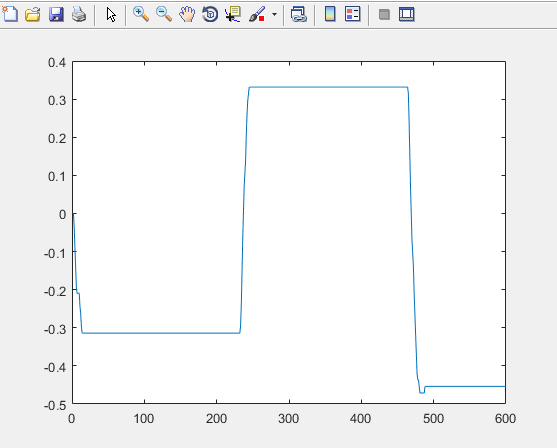
\includegraphics[width = 300pt]{figur/system_respons}
	\caption{System Respons}
	\label{fig:system_respons}
\end{figure}


Overføringsfunktionen bliver genereret ud fra funktionen \textit{tfest()}, som estimerer en overføring ud fra inputtet vs outputtet \textit{beta}. Hertil får vi overføringsfunktionen:

\begin{equation}
Tf(s) = \frac{5.029}{s^2 + 39.28 s + 717.9}
\end{equation}

\subsubsection{Pol placeringskontrol}
For at opfylde vores krav til dynamikken, forsøges der at placeres dominerede poler i systemet. Først findes damping ratio'en ($ \zeta $) ud fra valget om overshoot (OS) på følgende måde: 

\begin{equation}
\zeta = \frac{-\ln(OS/100)}{\sqrt{\pi^2+\ln^2(OS/100)}}
\end{equation} 

Dernæst findes båndbredden wn ud fra $ \zeta $ og valget om settling time (Ts) på følgede måde:

\begin{equation}
wn = \frac{4}{\zeta*Ts}
\end{equation} 

Til sidst kan den ønskede karakteristiske ligning (Gs) findes og ved:
\begin{equation}
G(s) = \frac{wn^2}{s^2+2*\zeta*wn*s+wn^2}
\end{equation}

Ud fra G(s) findes isoleres polerne, som skal bruges til at opfylde kravene om settling time (Ts) og overshoot (OS). For vores krav ligger polerne  derfor i -4\textpm\ 4.08i. For at fjerne steady state error tilføjes en ekstra pol i 5-10 gange real delen af de dominerende poler. Denne ekstra pol på reel aksen fungere som integrator i kontrolloopet, som korrigerer steady state error'en, men den øger også ordenen af systemet.


\subsubsection{State space model}

I dette projekt bliver systemet controller del repræsenteret på controller state space form, dette gøres for at kunne ændre på state vectorerne, som ændres vha. gainblokke (K), som bliver tilføjet til systemet. For at transformere transferfunktionen til en state space model, laves en state space tranformation i matlab. State space formlen giver følgende state space repræsentation

\begin{enumerate}
	
	\item
	$
	A = 
	\begin{bmatrix}
	
	-39.2765 & -717.8563 \\
	1.0000     &    0
	\end{bmatrix}
	$
	\item
	$
	B = 
	\begin{bmatrix}
	
	1\\
	0
	\end{bmatrix}
	$    
	
	\item 
	$
	C = 
	\begin{bmatrix}
	
	0  &  5.0293
	\end{bmatrix}
	$    
	\item
	$
	D = 
	\begin{bmatrix}
	
	0  
	\end{bmatrix}
	$  
\end{enumerate}      
Som vist tidligere, er der fundet nogle poler, som ønskes realiseret. Derfor indsættes en K matrix, som skal placeres, i tilbagekoblingen for at opnå de ønskede poler i close-loopet, dette ses nedenunder. 

\begin{lstlisting}[frame=single]
K = place(A,B,poles);
AA = A-B*(K);
sys=ss(AA,B,C,D);
\end{lstlisting}

Herved vises closed loop repræsentationen, for controller design, ift. kravene på overshoot og settling time.\\


HEREFTER KAN VI TILFØJE EN Ke, som regulerer på STEADY STATE ERROR (MANGLER KODE HERFRA). 



\subsection{Observer design}
Da systemet i praksis foregår på en motorblok, kan vi ikke hente de states matrixen, da x1 og x2 er en del  af systemet, ift ligningen for state space controller repræsentationen: 
\begin{gather}
\dot{x}=Ax+Bu \\
y=Cx
\end{gather}
Derfor indsættes yderligere en blok i systemet, for at kunne observere ind og output, og på baggrund af dem, og de beregnede state matrixes, beregnes en estimeret xhat, som skal bruges til tilbagekoblingen, som erstatning for states matrixen \\
Observer formlen hedder:


\begin{gather}
\dot{\hat{x}}=A\hat{x}+Bu+L(y-\hat{y}) \\
\hat{y}=C\hat{x}
\end{gather}

Vha af mellemregninger, får vi formlen: 
\begin{gather}
\dot{\hat{x}}=(A+BK-LC)\hat{x}+Ly \\
u=K\hat{x}
\end{gather}

Som er den formlen vi bruger til at lave vores observer.\\

Til observer tilføres en ny konstant L, som er udregnet til at styre observerens hastighed, så den er hurtigere end controlleren. L er beregnet ud fra formlen:
\begin{lstlisting}[frame=single]
L=place(A', C', poles)'
\end{lstlisting}

som er fundet her HENVISNING!!!

\subsection{Diskret controller design}
For at kunne implementere systemet på en microcontroller - som på LEGO EV3, kan systemet med fordel transformeres til en diskret state space model. Dette kommer af at reguleringen skal foregå på et digitalt system, som sampler med en bestemt frekvens. Både overføringsfunktionen og state space repræsentationen bliver transformeret til diskrete værdier, det samme gøres ved vores poler, hvormed K værdierne ændres til de passende værdier. Alt dette gøres igennem matlab, hvor funktionen c2d bliver brugt.


